
%(BEGIN_QUESTION)
% Copyright 2014, Tony R. Kuphaldt, released under the Creative Commons Attribution License (v 1.0)
% This means you may do almost anything with this work of mine, so long as you give me proper credit

In this system, a pair of line current differential relays (87) provide protection for a power line, each relay sensing current through the three line conductors at each end.  The optional slash mark and ``$I_A$, $I_B$, $I_C$'' notations emphasize the fact that the relays are monitoring all three phases:

$$\includegraphics[width=15.5cm]{i00852x01.eps}$$

Suppose a line-to-line fault develops between phases A and B of this power line, with no connection whatsoever to earth ground.  Determine whether or not the 87 relays will trip, and explain why.  

\underbar{file i00852}
%(END_QUESTION)





%(BEGIN_ANSWER)

A fault between A and B phases will cause current to branch from both of these conductors at the point of the fault.  This will create current imbalances between the far ends (CT measurement points) on A phase as well as on B phase, telling the relays there is a differential current problem in the line.

\vskip 10pt

A diagram showing an instantaneous view of current (taken at some moment in time) shows the discrepancies in current for both phases:

$$\includegraphics[width=15.5cm]{i00852x02.eps}$$

Given some nontrivial amount of fault current $I_F$, the currents measured at both ends of A phase are clearly unequal ($I_A \neq I_A - I_F$).  Likewise for B phase: ($I_B \neq I_B + I_F$).  Thus, the two 87 relays comparing currents for each phase at both ends of the power line will be able to tell there is a line-to-line fault somewhere between the CT sets.

%(END_ANSWER)





%(BEGIN_NOTES)


%INDEX% Protective relay: differential current (87)

%(END_NOTES)

